\tikzset{
  basic/.style  = {draw, text width=2cm, rectangle},
  root/.style   = {basic, rounded corners=2pt, thin, align=center, fill=gray!30},
  level 2/.style = {basic, rounded corners=2pt, thin, align=center, text width=5.5em},
  level 3/.style = {basic, dashed, align=center, text width=4.5em, fill=gray!30},
  level 4/.style = {basic, rounded corners=6pt, thin, align=center}
}

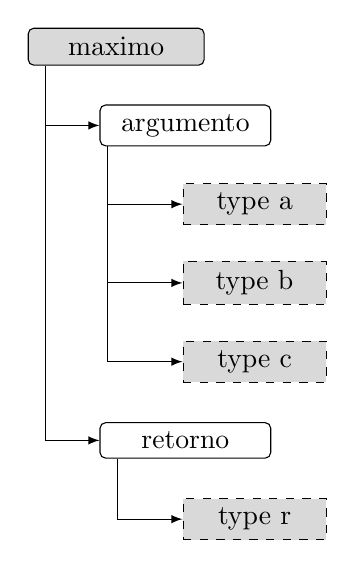
\begin{tikzpicture}[
  level 1/.style={sibling distance=40mm},
  edge from parent/.style={->,draw},
  >=latex, level distance=1.8cm]

\node[root] (c2) {maximo};

% The second level, relatively positioned nodes
\begin{scope}[every node/.style={level 2}]
\node [below of = c2, xshift=25pt] (c21) {argumento};
\end{scope}

\begin{scope}[every node/.style={level 3}]
\node [below of = c21, xshift=25pt] (c211) {type a};
\node [below of = c211] (c212) {type b};
\node [below of = c212] (c213) {type c};
\end{scope}

\begin{scope}[every node/.style={level 2}]
\node [below of = c213, xshift=-25pt] (c22) {retorno};
\end{scope}

\begin{scope}[every node/.style={level 3}]
\node [below of = c22, xshift=25pt] (c221) {type r};
\end{scope}

\foreach \value in {1,...,2}
  \draw[->] (c2.195) |- (c2\value.west);

\foreach \value in {1,...,3}
 \draw[->] (c21.195) |- (c21\value.west);

\foreach \value in {1}
 \draw[->] (c22.195) |- (c22\value.west);

\end{tikzpicture}